\documentclass[]{article}
\usepackage{amssymb,latexsym,amsmath}     % Standard packages
\usepackage[pdftex]{graphicx}
\usepackage{subcaption}

\addtolength{\textwidth}{1.0in}
\addtolength{\textheight}{1.00in}
\addtolength{\evensidemargin}{-0.75in}
\addtolength{\oddsidemargin}{-0.75in}
\addtolength{\topmargin}{-.50in}
\usepackage[lf]{venturis}
\usepackage[T1]{fontenc}
% \usepackage{newtxtext,newtxmath}
% \renewcommand{\familydefault}{\sfdefault}  % sans-serif!


\usepackage{fancyhdr}
\renewcommand\headrule{}
\pagestyle{fancy}
\makeatletter
\let\ps@plain\ps@fancy % make plain pages fancy
\makeatother
\fancyhf{}
\lhead{\textbf{Rhythm Knights}\\
Gameplay Specification}
\rhead{\resizebox{0.75in}{!}{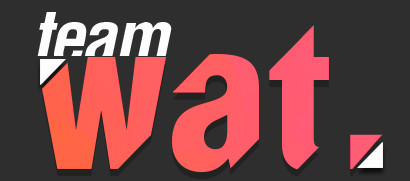
\includegraphics{img/logo_team.jpg}}}
\rfoot{\thepage}

\begin{document}

\title{\textbf{Rhythm Knights} \\ Concept Document}
\author{Team \emph{wat} \\
\small{Kylar Henderson, Charles Tark, 
Gagik Hakobyan, Julia Cole, Andrew Halpern, Austin Liu}}
\date{} % removed date
\maketitle

\section*{High Concept Statement}
You arrive at a dance party fashionably late and realize something is
amuck. All of the other party attendees have been turned into monster
zombies because of the music being played by the evil DJ. You must
withstand hordes of monsters to reach the DJ and save them all with
the power of music.

\section*{Features}
\begin{itemize}
\item Time your actions to the beat to build up combos and score points
\item Slash through hordes of enemies with your trusty neon saber
\item Dash over perilous pits to cross the dancefloor
\item Shoot glowing projectiles to defeat enemies
\item Freeze enemies in their tracks
\end{itemize}

\section*{Design Goals}
\begin{itemize}
\item
  \textbf{Rhythm Centric Combat} - The goal of the game is to test the
  players' abilities to follow along with the rhythm of the music. The
  players should feel like they are at a wacky 21st century dance party
  and the combination of techno music and rhythm based combat is geared
  towards a younger audience attracted to electronic dance music.
\item
  \textbf{Play Style} - Players must react quickly to changes in the
  music and the environment around them. The game emphasizes timing
  accuracy, long combo streaks, and short-down time between objectives.
\end{itemize}

\pagebreak
\section*{Market Segment}
\subsection*{Genre}
This is an action rhythm game. The players must defeat enemies by 
timing their actions to the displayed beat sequence. 

\subsection*{Platform}
Rhythm Knights is designed for the desktop and will be played with a keyboard. 
It is also recommended that players have headphones for optimal danciness. 

\subsection*{Competition}
\begin{itemize}
\item Dance Dance Revolution (series): DDR's mechanics involve hitting
  keys to the beat of the music and the players must match a specific
  key pattern to progress through the level. In its core, this is one of
  the main mechanics of our game.
\item Guitar Hero (series): Similarly to DDR, Guitar Hero involves
  matching a key pattern to the beat of the music, so we again have an
  overlap of mechanics.
\item This is probably the main competition for our game. Crypt of the
  Necrodancer has similar themes. It is a game about fighting monsters
  while confined to a rhythm. However, Crypt of the Necrodancer focuses
  on exploration and Rogue-like elements, while Rhythm Knights focuses on
  puzzle elements and consistently acting on a different beat for each
  level.
\end{itemize}
\subsection*{Unique Selling Points}
There will be different genres of music for each level using unique
rhythms on dance floor environments inspired by the world. Some levels
will have a more basic map and a complicated rhythm, while others will
have a more complex map and a basic rhythm. A different beat style in
each level will make for a new experience every time. The game's
rhythm ``ticker'' will dictate what actions players are allowed to
perform on a given beat. Players will also be given the choice of
special abilities such as dashing, freezing, and shooting on certain
beats of the music.


\pagebreak
\section*{Gameplay Sketches}
\begin{figure}[!htb]
\begin{center}
\leavevmode
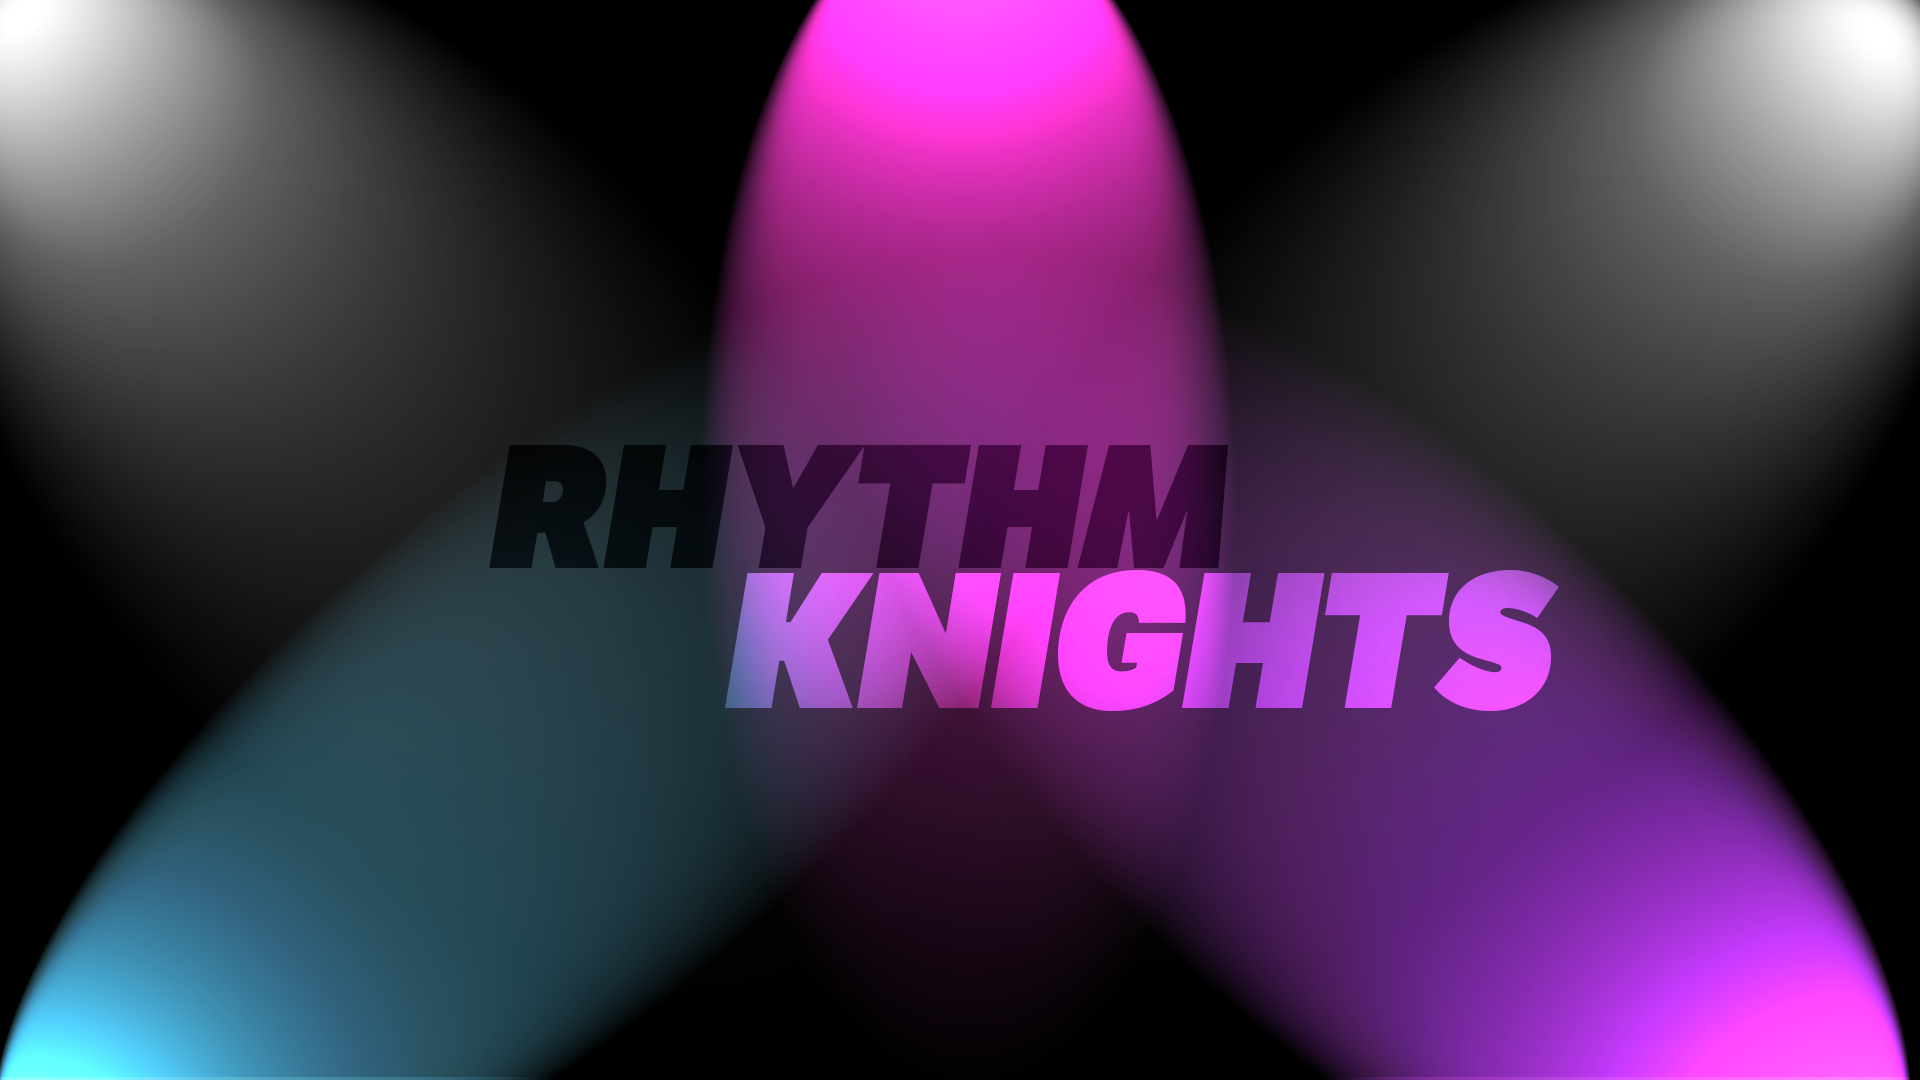
\includegraphics[width=4.7in]{img/splash.jpg}
\end{center}
\caption{Current splash screen for Rhythm Knights \label{splashscreen}}
\end{figure}

\begin{figure}[htb!]
\begin{subfigure}{.5\textwidth}
  \centering
  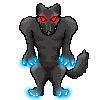
\includegraphics[width= 1.5in]{img/enemy_front.jpg}
  \caption{Front view of enemy
  \label{en_front}}
\end{subfigure}%
\begin{subfigure}{.5\textwidth}
  \centering
  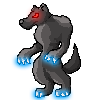
\includegraphics[width=1.5in]{img/enemy_side.jpg}
  \caption{Side view of enemy
  \label{en_side}}
\end{subfigure}%
\caption{Enemy views
\label{enemy}}
\end{figure}


\begin{figure}[!htb]
\begin{center}
\leavevmode
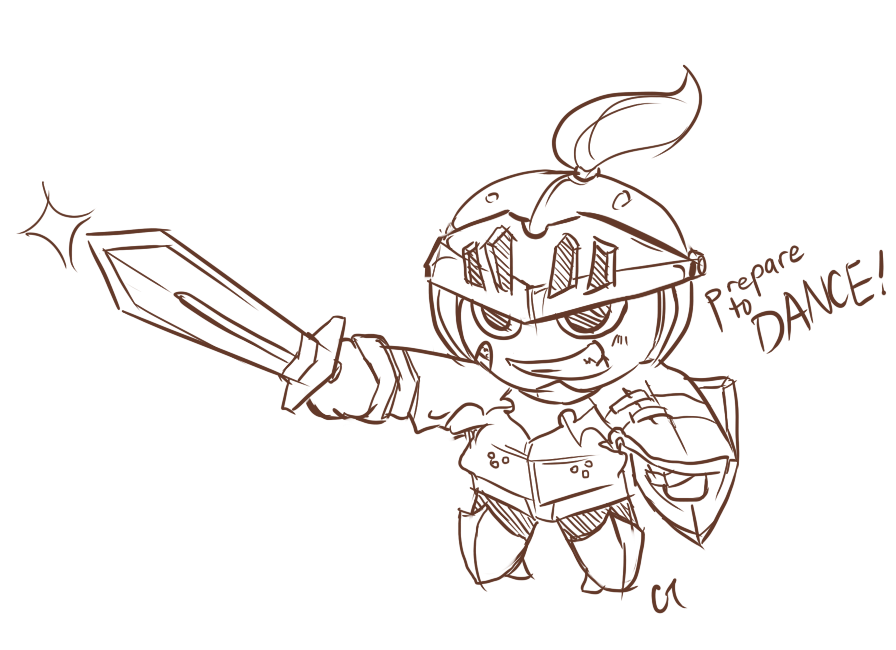
\includegraphics{img/main_char.jpg}
\end{center}
\caption{A sketch of our main character \label{logo}}
\end{figure}


\begin{figure}[!htb]
\begin{center}
\leavevmode
\resizebox{4.7in}{!}{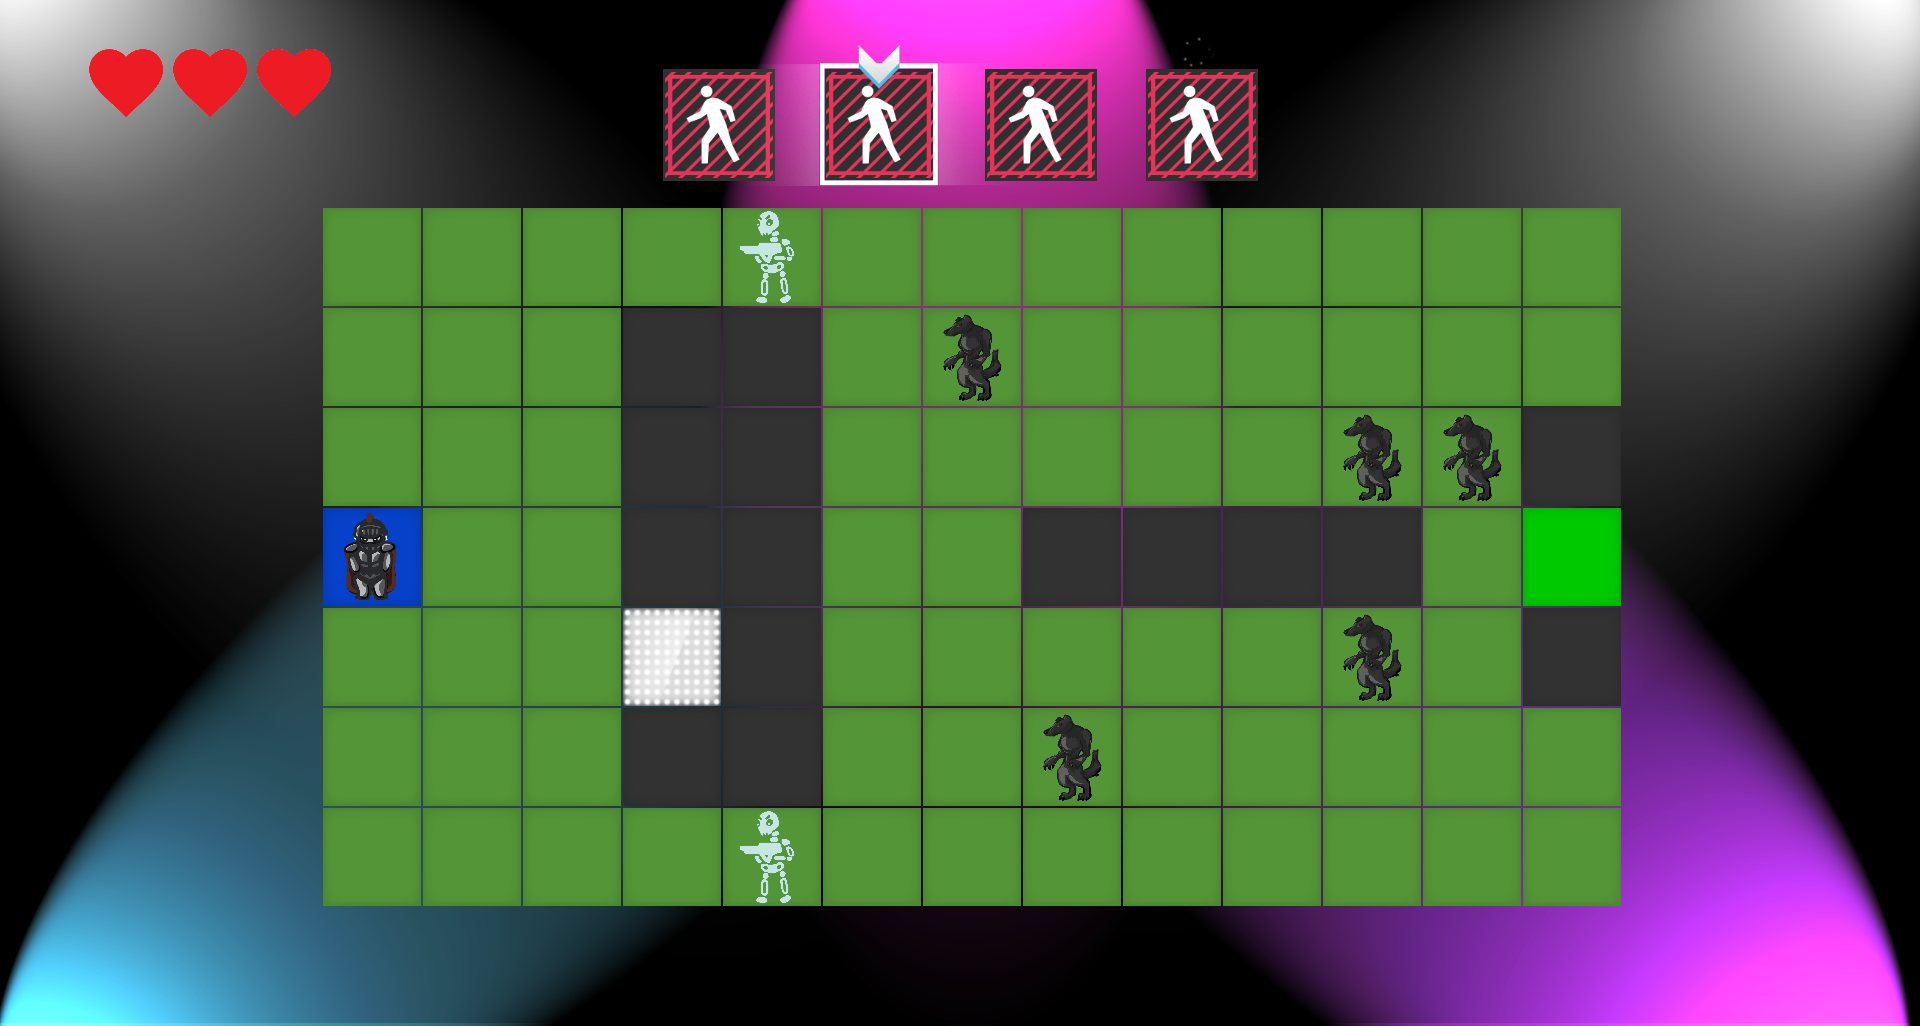
\includegraphics{img/play_screen.jpg}}
\end{center}
\caption{ This is a rough example of what levels will look like
(currently with placeholder assets). Black tiles represent obstacles
that cannot be stepped on, but can be dashed over. White tiles will
move along a set path and players can ride them for as long as they
like. The ticker at the top of the map indicates the full beat
sequence for the level as well as the current action players must
make.\label{play_sketch}}
\end{figure}

\end{document}
